\chapter{Explorative Datenanalyse}
Die nachfolgenden Abbildungen beziehen sich auf die Versuchsperson 001.\\
Abbildung \ref{fig:AugenX-Positionen} zeigt die x-Position des Blicks vom linken Auge auf der x-Achse und die x-Position des Blicks des rechten Auges auf der y-Achse. Die schwarze Linie markiert die Stellen, wo beide Augen auf der x-Position auf die gleiche Stelle geschaut haben. Die Farbskala geht von blau nach rot und zeigt den zeitlichen Verlauf.\\
Bei allen Punkten \"uber der Linie hat das rechte Auge weiter nach rechts geblickt, als das linke. Bei allen Punkten unterhalb der Linie war es umgekehrt.

\begin{figure}[H]
	\noindent \begin{centering}
		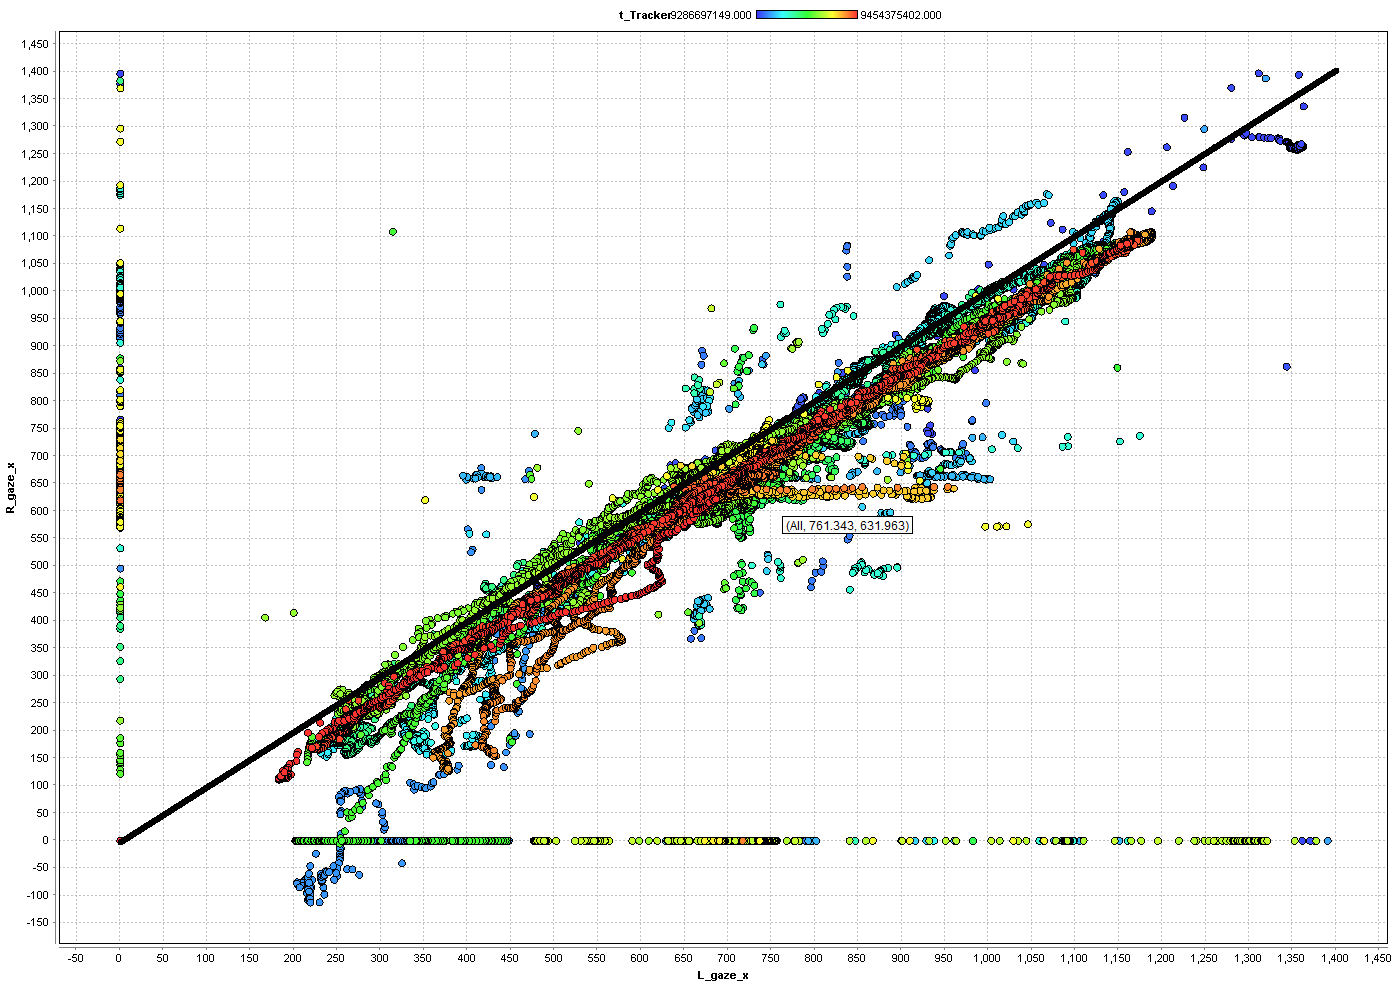
\includegraphics[width=15cm]{pics/Augen-X-Positionen.png}
		\par\end{centering}
	\caption{\label{fig:AugenX-Positionen}Vergleich der x-Werte der Blickposition beider Augen \cite{BilderExplorativeDatenanalyseBoersch}}
\end{figure}

Abbildung \ref{fig:BlickeLinkesAuge} zeigt die Blickposition des linken Auges. Dabei wird die x-Position auf der x-Achse dargestellt und die y-Position auf der y-Achse. Abbildung \ref{fig:BlickeRechtesAuge} zeigt die Blickposition des rechten Auges. Die Achsenbelegung ist gleich.\\
Es wird deutlich, dass sich die Blickpositionen der beiden Augen voneinander unterscheiden.

\begin{figure}[H]
	\noindent \begin{centering}
		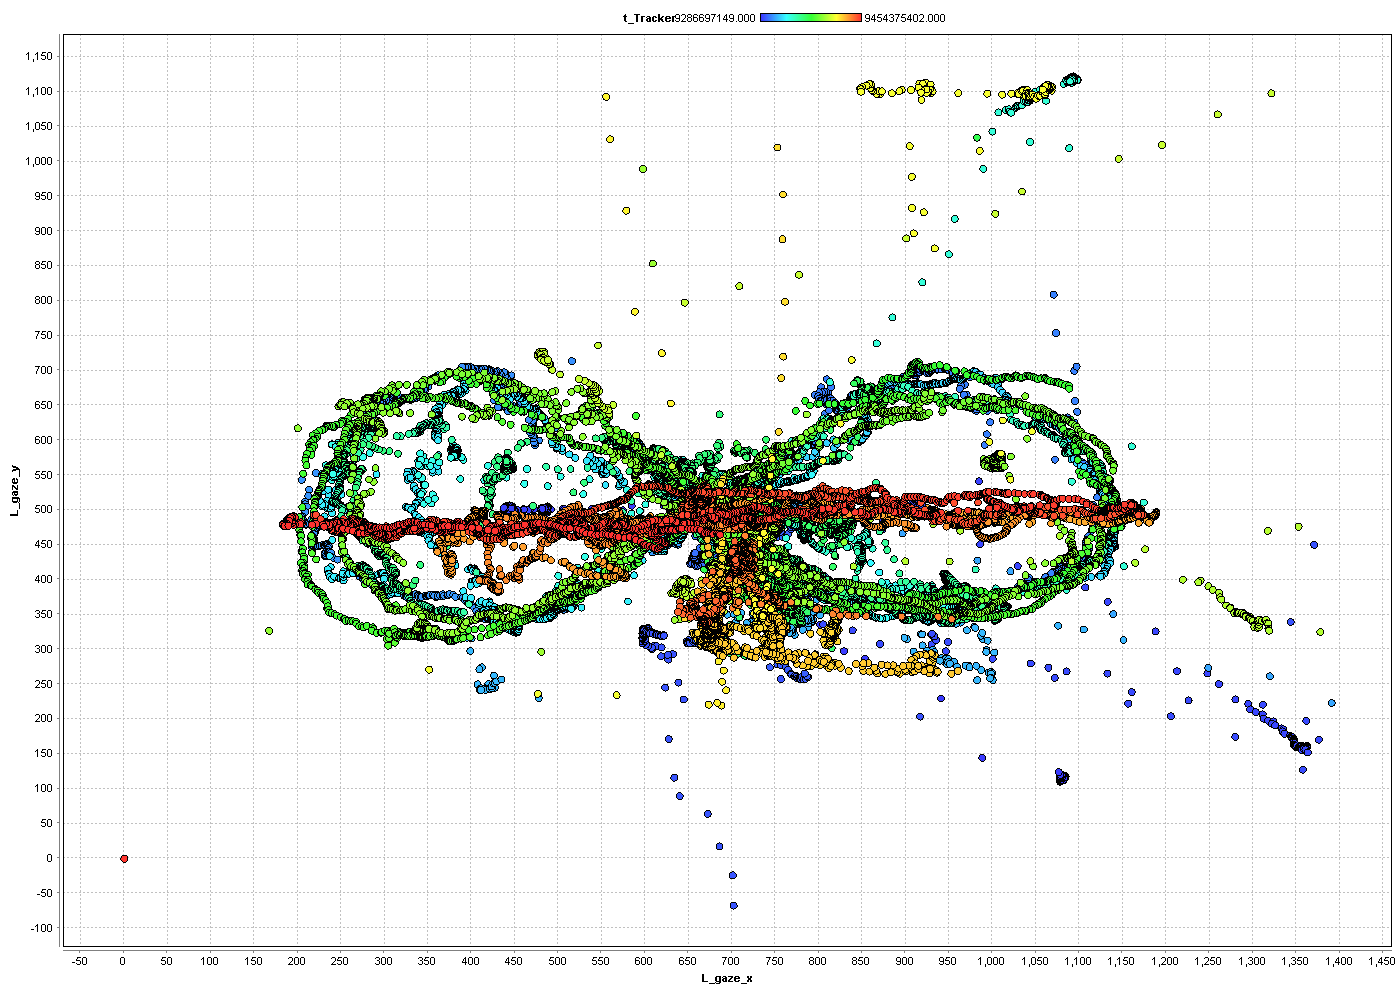
\includegraphics[width=15cm]{pics/BlickeLinkesAuge.png}
		\par\end{centering}
	\caption{\label{fig:BlickeLinkesAuge}Blickpositionen linkes Auge \cite{BilderExplorativeDatenanalyseBoersch}}
\end{figure}

\begin{figure}[H]
	\noindent \begin{centering}
		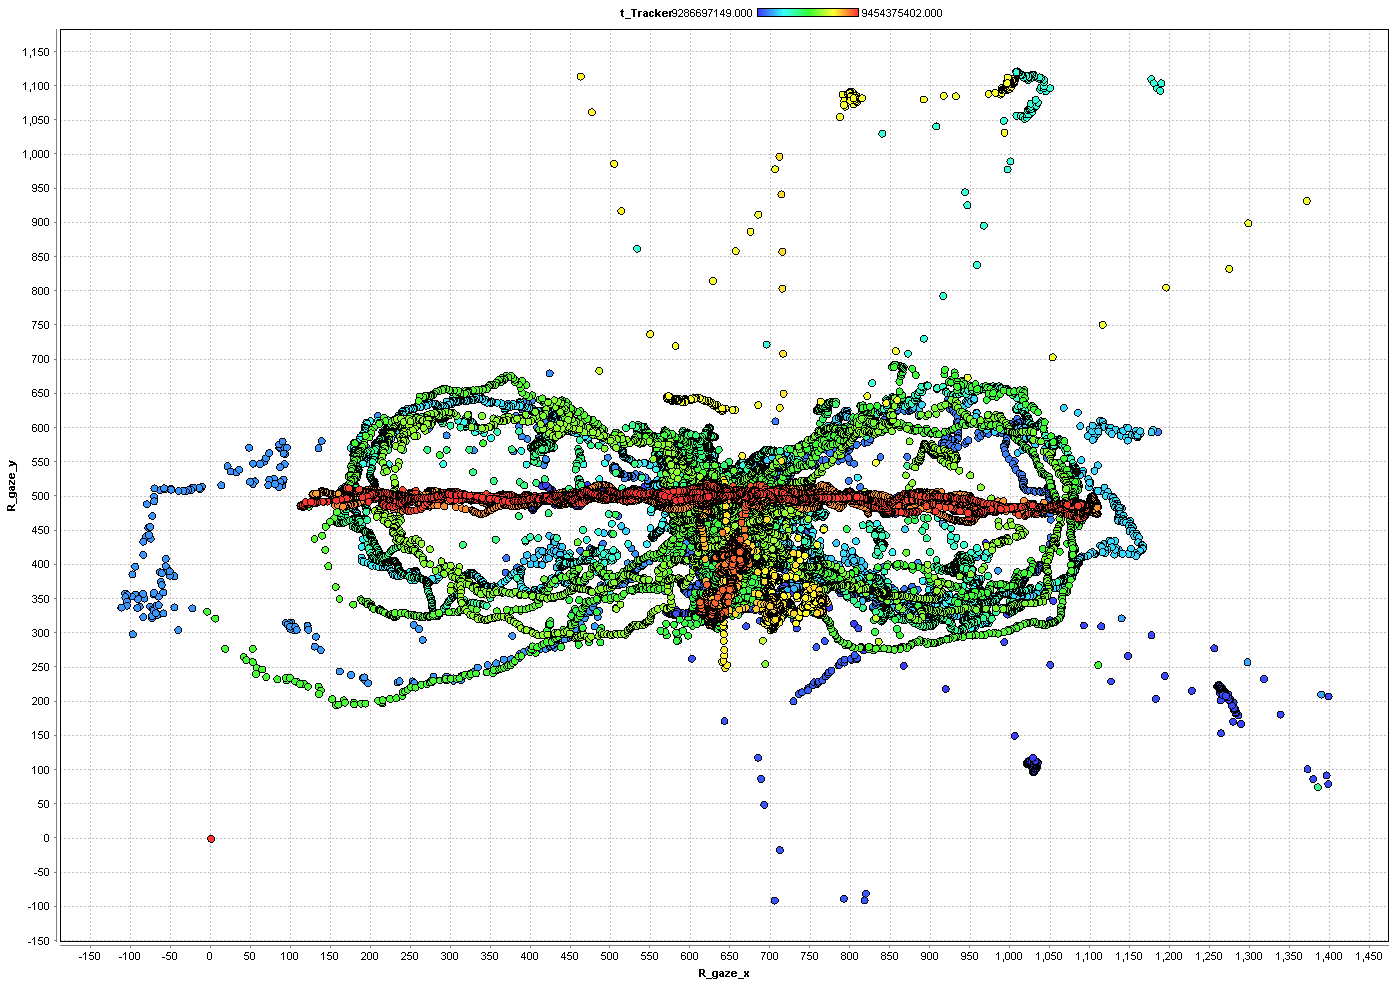
\includegraphics[width=15cm]{pics/BlickeRechtesAuge.png}
		\par\end{centering}
	\caption{\label{fig:BlickeRechtesAuge}Blickpositionen rechtes Auge \cite{BilderExplorativeDatenanalyseBoersch}}
\end{figure}

Abbildung \ref{fig:OuterJoin} zeigt einen Outer join, \"uber die Zeitwerte der Targetdatei und der Blickdatei. Dadurch ist zu erkennen, dass die beiden Dateien keine bzw. kaum gleiche Zeitwerte aufweisen. Au\ss{}erdem ist zu sehen, dass die Blickwerte etwa vier mal so oft gemessen wurden, als die Targetwerte.

\begin{figure}[H]
	\noindent \begin{centering}
		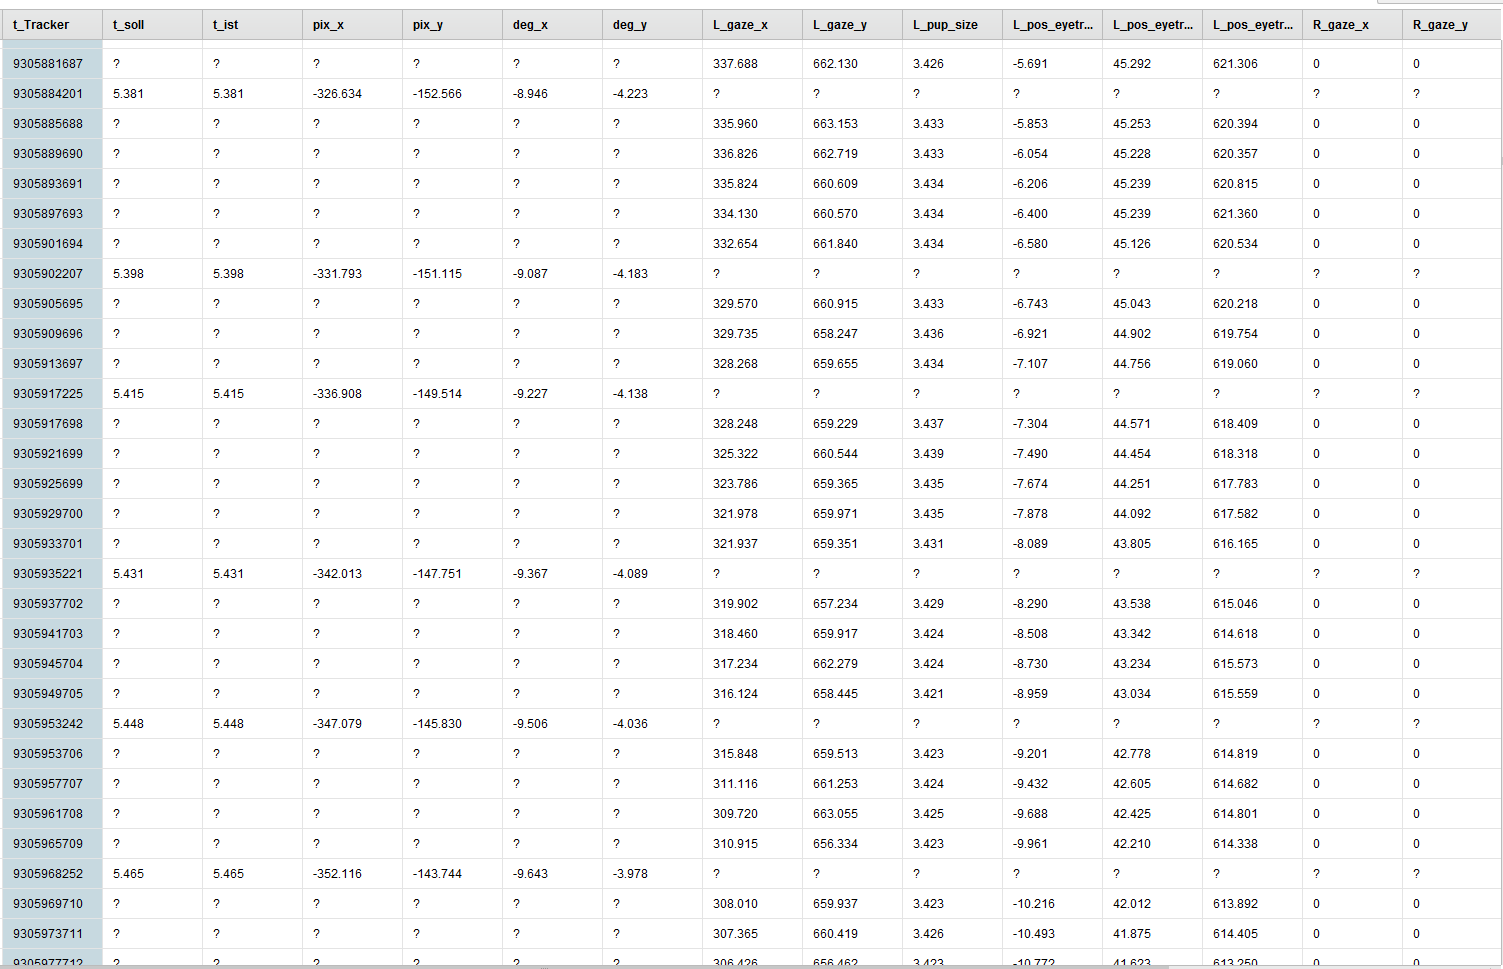
\includegraphics[width=15cm]{pics/OuterJoin.png}
		\par\end{centering}
	\caption{\label{fig:OuterJoin}Outer Join Targetwerte und Blickwerte \"uber Zeitstempel \cite{BilderExplorativeDatenanalyseBoersch}}
\end{figure}

Die Histogramme in Abbildung \ref{fig:HistogrammZeitenTargetdateien} und Abbildung \ref{fig:HistogrammZeitenBlickdateien} stellen die Verteilung der Werte der Zeitabst\"ande der Targetdatei und der Blickdatei dar. Dadurch wird deutlicher, wie gro\ss{} der Unterschied zwischen der Anzahl der Messungen ist.

\begin{figure}[H]
	\noindent \begin{centering}
		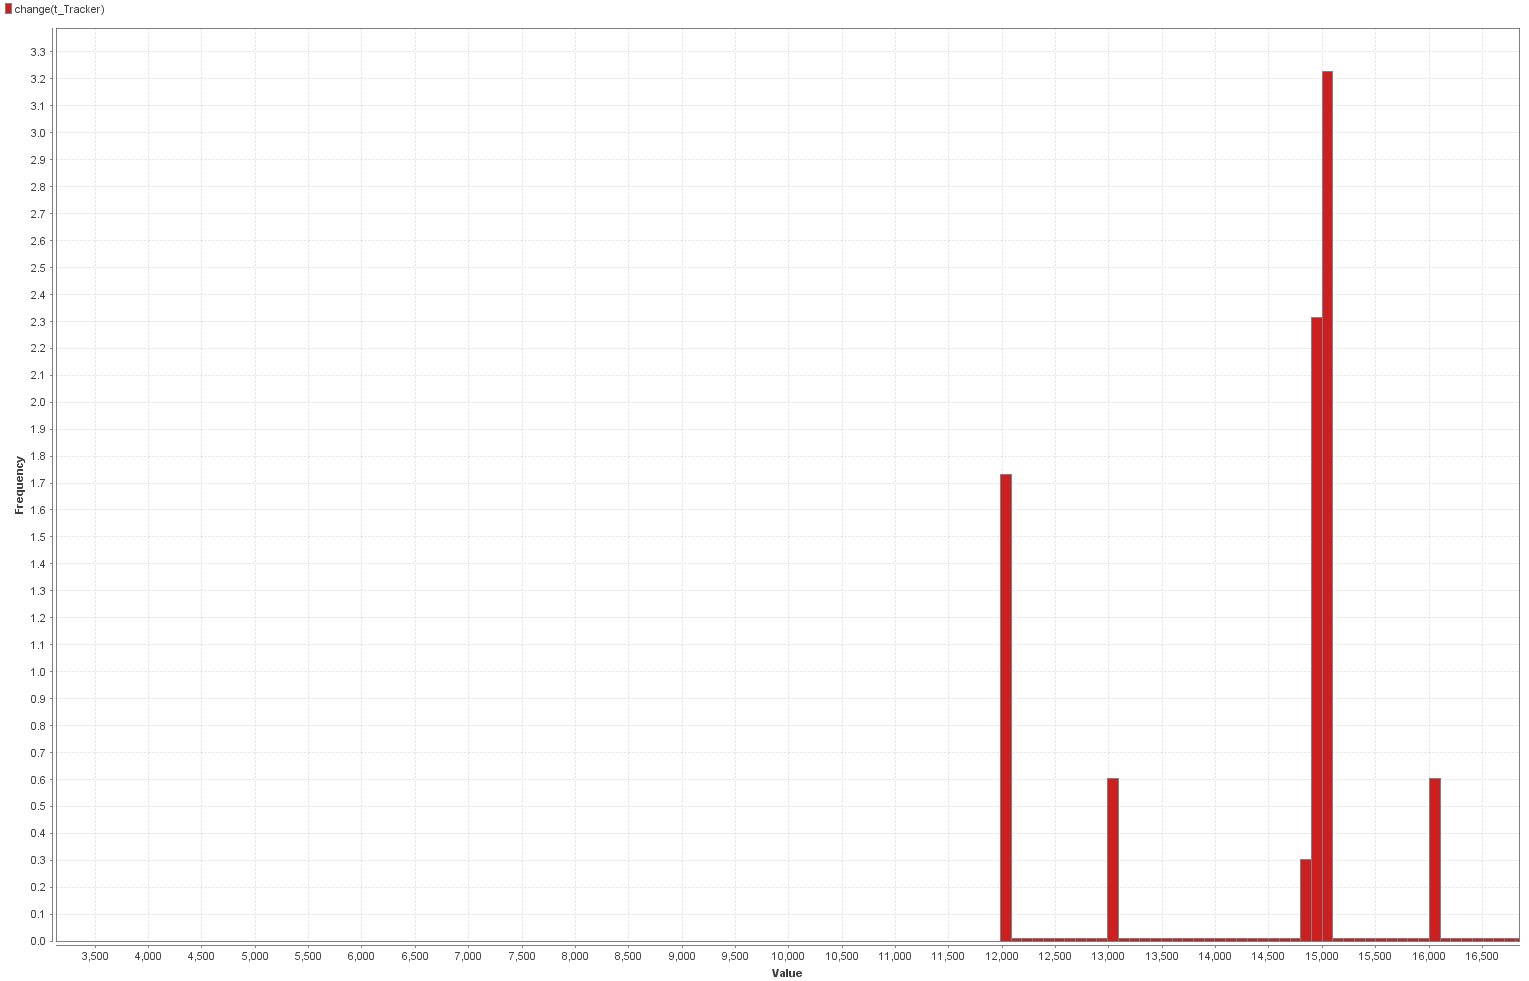
\includegraphics[width=15cm]{pics/HistogrammZeitenTargetdateien.png}
		\par\end{centering}
	\caption{\label{fig:HistogrammZeitenTargetdateien}Histogramm Zeitabst\"ande der Messungen Targetdatei \cite{BilderExplorativeDatenanalyseBoersch}}
\end{figure}

\begin{figure}[H]
	\noindent \begin{centering}
		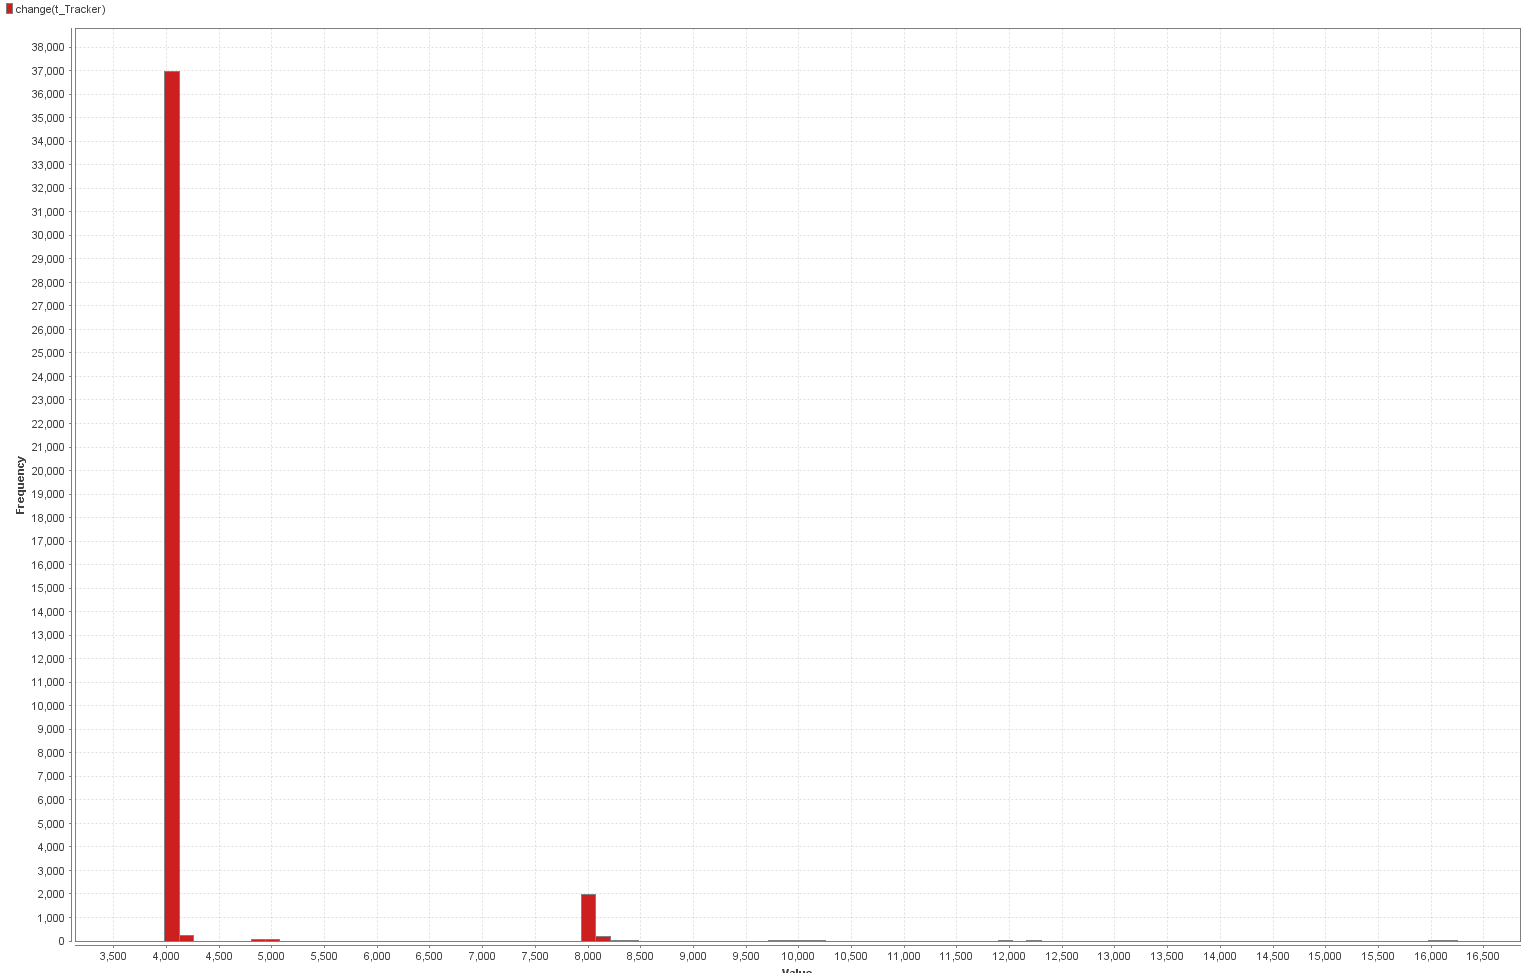
\includegraphics[width=15cm]{pics/HistogrammZeitenBlickdateien.png}
		\par\end{centering}
	\caption{\label{fig:HistogrammZeitenBlickdateien}Histogramm Zeitabst\"ande Messungen Blickdaten \cite{BilderExplorativeDatenanalyseBoersch}}
\end{figure}